\documentclass[aspectratio=169]{../latex_main/tntbeamer}  % you can pass all options of the beamer class, e.g., 'handout' or 'aspectratio=43'
\usepackage{dsfont}
\usepackage{bm}
\usepackage[english]{babel}
\usepackage[T1]{fontenc}
%\usepackage[utf8]{inputenc}
\usepackage{graphicx}
\graphicspath{ {./figures/} }
\usepackage{algorithm}
\usepackage[ruled,vlined,algo2e,linesnumbered]{algorithm2e}
\usepackage{hyperref}
\usepackage{booktabs}
\usepackage{mathtools}

\usepackage{amsmath,amssymb}
\usepackage{latexsym}

\DeclareMathOperator*{\argmax}{arg\,max}
\DeclareMathOperator*{\argmin}{arg\,min}

\usepackage{pgfplots}
\pgfplotsset{compat=1.16}
\usepackage{tikz}
\usetikzlibrary{trees} 
\usetikzlibrary{shapes.geometric}
\usetikzlibrary{positioning,shapes,shadows,arrows,calc,mindmap}
\usetikzlibrary{positioning,fadings,through}
\usetikzlibrary{decorations.pathreplacing}
\usetikzlibrary{intersections}
\pgfdeclarelayer{background}
\pgfdeclarelayer{foreground}
\pgfsetlayers{background,main,foreground}
\tikzstyle{activity}=[rectangle, draw=black, rounded corners, text centered, text width=8em]
\tikzstyle{data}=[rectangle, draw=black, text centered, text width=8em]
\tikzstyle{myarrow}=[->, thick, draw=black]

% Define the layers to draw the diagram
\pgfdeclarelayer{background}
\pgfdeclarelayer{foreground}
\pgfsetlayers{background,main,foreground}

\input{./latex_main_old/macros}

% Requires XeLaTeX or LuaLaTeX
\usepackage{unicode-math}

\usepackage{fontspec}
%\setsansfont{Arial}
\setsansfont{RotisSansSerifStd}[ 
Path=./latex_main/fonts/,
Extension = .otf,
UprightFont = *-Regular,  % or *-Light
BoldFont = *-ExtraBold,  % or *-Bold
ItalicFont = *-Italic
]
\setmonofont{Cascadia Mono}[
Scale=0.8
]

% scale factor adapted; mathrm font added (Benjamin Spitschan @TNT, 2021-06-01)
%\setmathfont[Scale=1.05]{Libertinus Math}
%\setmathrm[Scale=1.05]{Libertinus Math}

% other available math fonts are (not exhaustive)
% Latin Modern Math
% XITS Math
% Libertinus Math
% Asana Math
% Fira Math
% TeX Gyre Pagella Math
% TeX Gyre Bonum Math
% TeX Gyre Schola Math
% TeX Gyre Termes Math

% Literature References
% #1 = Display Name
% #2 = Url (without \href)
\newcommand{\lit}[2]{\href{#2}{\footnotesize\color{black!60}[#1]}}

%%% Beamer Customization
%----------------------------------------------------------------------
% (Don't) Show sections in frame header. Options: 'sections', 'sections light', empty
\setbeamertemplate{headline}{empty}

% Add header logo for normal frames
\setheaderimage{
	% \includegraphics[height=\logoheight]{figures/TNT_darkv4.pdf}
	\includegraphics[height=\logoheight]{./latex_main/figures/luh_logo_rgb_0_80_155.pdf}
	% \includegraphics[height=\logoheight]{figures/logo_tntluh.pdf}
}

% Header logo for title page
\settitleheaderimage{
	% \includegraphics[height=\logoheight]{figures/TNT_darkv4.pdf}
	\includegraphics[height=\logoheight]{./latex_main/figures/luh_logo_rgb_0_80_155.pdf}
	% \includegraphics[height=\logoheight]{figures/logo_tntluh.pdf}
}

% Title page: tntdefault 
\setbeamertemplate{title page}[tntdefault]  % or luhstyle
% Add optional title image here
%\addtitlepageimagedefault{\includegraphics[width=0.65\textwidth]{figures/luh_default_presentation_title_image.jpg}}

% Title page: luhstyle
% \setbeamertemplate{title page}[luhstyle]
% % Add optional title image here
% \addtitlepageimage{\includegraphics[width=0.75\textwidth]{figures/luh_default_presentation_title_image.jpg}}

\author[Lindauer]{Marius Lindauer\\[1em]
	\includegraphics[height=\logoheight]{./latex_main/figures/luh_logo_rgb_0_80_155.pdf}\qquad
\includegraphics[height=\logoheight]{./latex_main/figures/TNT_darkv4}\qquad
\includegraphics[height=\logoheight]{./latex_main/figures/L3S.jpg}	}
\date{Winter Term 2021
}


%%% Custom Packages
%----------------------------------------------------------------------
% Create dummy content
\usepackage{blindtext}

% Adds a frame with the current page layout. Just call \layout inside of a frame.
\usepackage{layout}


\usepackage[usenames,dvipsnames]{xcolor}
\usepackage{pgf-pie} 
\newcommand{\todo}[1]{
	% Die folgende Zeile kann auskommentiert werden, um die ToDo's zu entfernen
	\textcolor{red}{[\textbf{ToDo}: \emph{#1}]}
}

\title[Conclusion]{RL: Projects 2022/23}
\subtitle{}

%\institute{}


\begin{document}
	
	\maketitle

	%-----------------------------------------------------------------------------------------------------------------------------

\begin{frame}[c]{Grading Scheme: 1-Student Team (Project)}
 
	\begin{itemize}
		\item Up to 25 points for working on the project; Should include:
        \begin{enumerate}
            \item Implementation of the approach: 10 points
            \begin{itemize}
                \item See next slides for details
            \end{itemize}
            \item Evaluation of the approach: 5 points
            \item Gained insights: 5 points
            \item Extras, e.g, ablation study, extensions, variations, ...: 5-20 points
        \end{enumerate}
            \item[$\leadsto$] We expect at least 15 points from working on your project; otherwise, we consider the entire exam as failed
            \item[$\leadsto$] You can get up to 15 bonus points by exceeding our expectations (e.g., see ``Extras'' above and ``Further goals'' on the next slides)
            \item \alert{Write a proposal (at most 1 page) outlining the above points with concrete ToDos and upload it to GitHub Classroom by Tuesday, Jan  at 15:00}
        \end{itemize}
        
\end{frame}

%----------------------------------------------------------------------
\begin{frame}[c]{Track I: New Env}
	
	\begin{itemize}
		\item Propose a new \& interesting benchmark environment / application for RL (incl. state, action, reward, transition, $\ldots$)
		\begin{itemize}
			\item Use Gymnasium env API
			\item \alert{Has to be related to preventing climate change / Green AI}
		\end{itemize}
		\item Minimal requirement: An RL agent (of your choice) can learn something reasonable
		\begin{itemize}
			\item That is, it performs better than a static and random policy
			\item You can use SAC from stable-baselines as an implemented RL algorithm to train an agent
			\item In addition, you can also evaluate PPO, DQN or other state-of-the-art baselines
		\end{itemize}
		\item Further goals could include:
		\begin{itemize}
			\item Impact of state or action space (e.g., size or encoding)
			\item Reward signal or reward shaping
			\item Does the Markov assumption hold true?
		\end{itemize}
		\item[$\leadsto$] Environment should not be too trivial (e.g., a small maze)
	\end{itemize}
	
\end{frame}
%----------------------------------------------------------------------
%----------------------------------------------------------------------
\begin{frame}[c]{Track II: RL Agent}
	
	\begin{itemize}
		\item Implement an RL agent from scratch
		\begin{itemize}
		    \item Pick a (recent) RL paper and re-implement it OR extend an existing algorithm with a (recent) idea
			\item Don't use existing implementations!
		\end{itemize}
		\item Minimal requirement: Your RL agent can learn a reasonable policy\\ on an RL benchmark of your choice
		\begin{itemize}
			\item That is, it performs better than a static or random policy
			\item You have to evaluate it on \url{https://github.com/rte-france/Grid2Op}
		\end{itemize}
		\item Further goals could include:
		\begin{itemize}
			\item Variants of different algorithm components (e.g., experience replay)
			\item Hyperparameter sensitivity study
			\item Comparison against other baselines
		\end{itemize}
	\end{itemize}
	
\end{frame}
%----------------------------------------------------------------------
\begin{frame}[c]{Grading Scheme: 1-Student Team (Presentation and Q\,\&\,A)}

\begin{itemize}
\medskip
		\item Up to 25 points for presenting the results (10min presentation + 5min Q\,\&\,A)
            \begin{itemize}
                \item at most 7 slides (without title slide) are allowed
                \item Concise and convincing presentation of the approach, your ideas, and the interpretation of the results
                \item Good illustrations and figures
                \item Point reductions for unreadable slides and too-small font sizes
                \item recommended: \url{https://youtu.be/IJw8q3gNqeI}
            \end{itemize}
\end{itemize}
\end{frame}

\begin{frame}[c]{Grading Scheme: 1-Student Team (Lecture Knowledge)}


\begin{columns}

\column{0.6\textwidth}

\vspace*{-2.3em}
   \begin{itemize}
		\item Up to 50 points for Q\,\&\,A about the lecture content (15min)
            \begin{itemize}
                \item Know everything from the lecture
            \end{itemize}
             
		\item[$\leadsto$] 100 points overall
		\begin{itemize}
		    \item bonus points on top
		\end{itemize}
		\medskip
		\item Points translation to grades:
		\begin{itemize}
		    \item 4.0: $\geq$ 45 points (3.7: $\geq$ 50, 3.3: $\geq$ 55)
		    \item 3.0: $\geq$ 60 points (2.7: $\geq$ 65, 2.3: $\geq$ 70)
		    \item 2.0: $\geq$ 75 points (1.7: $\geq$ 80, 1.3: $\geq$ 85)
    		\item 1.0: $\geq$ 90 points
		\end{itemize}
		\medskip
            \pause
		\item \alert{For each additional team member (max. 3 students per team), $+5$ points for minimal project points and points-grades translation, $+10$ min exam}
	\end{itemize}

\column{0.4\textwidth}

\scalebox{0.8}{
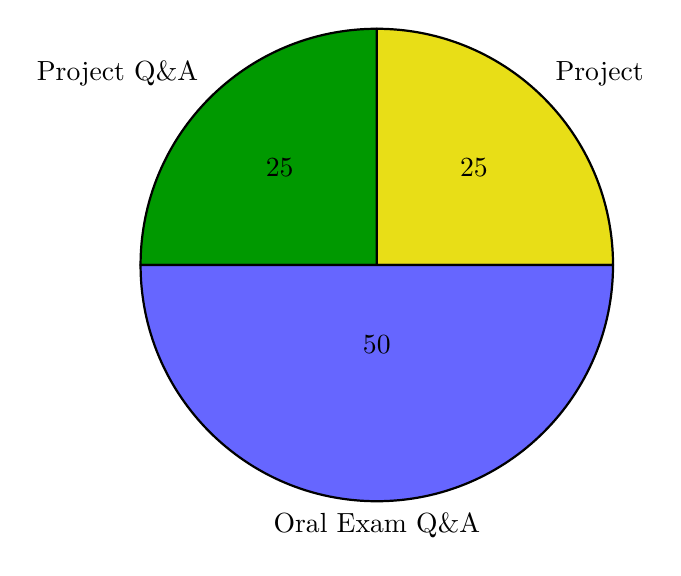
\begin{tikzpicture}


\pie[
    color = {
        yellow!90!black,
        green!60!black,
        blue!60}, 
    sum = auto
]{25/Project,
    25/Project Q\&A,
    50/Oral Exam Q\&A
}
 
\end{tikzpicture}
}

\end{columns}
     
\end{frame}

\begin{frame}[c]{Further Requirements}
 
	\begin{itemize}
		\item clean code (-5 points if not available)
		\item well documented (-5 points if not available)
		\item unit tested (-5 points if not available)
		\item all requirements well documented (e.g., requirements.txt) (-5 points if not available)
		\item README.md file with installation instructions (-5 points if not available)
		\item Reproducible results\footnote{\url{https://docs.google.com/document/d/1Us7LqPIpH4wkbKWhyK8N_rICylv4Hqob9gzUi01VU18/edit?usp=sharing}}, e.g., running with several random seeds (-5 points if not ensured)
            \begin{itemize}
                \item Document everything in your GitHub repo!
            \end{itemize}
		\item Show-up at the exam (-100 points otherwise)
	\end{itemize}
	
\end{frame}

\begin{frame}[c]{Submission}
    \begin{itemize}
        \item Proposal Deadline: January 26th, 2022 at 15:00
        \begin{itemize}
            \item Submit via: \url{https://classroom.github.com/a/OLyBPe9o}
        \end{itemize}
        \item Appointment selection in StudIP: January 26th, 2023 at 18:00
        \item Submission Deadline: February 20th, 2023 at 18:00 (one week before the exam week)
        \begin{itemize}
            \item Submit via: \url{https://classroom.github.com/a/pdkEucBp}
        \end{itemize}
        \item Exam: February 27th - March 3rd 2023
    \end{itemize}
\end{frame}

	%-----------------------------------------------------------------------------------------------------------------------------
	%-----------------------------------------------------------------------------------------------------------------------------
    % Projects
	%-----------------------------------------------------------------------------------------------------------------------------


\begin{frame}[c]{Submission Date}

    \huge
    \begin{center}
	    February 20th 2023 at 18:00
    \end{center}
\end{frame}


\end{document}